\documentclass[a4paper]{article}
\usepackage{graphicx}
\usepackage{lipsum}
\usepackage{background}
\backgroundsetup{
  scale=4.9,
  angle=90,
  opacity=0.9,
  contents={
\includegraphics{./FULLHOUSE/resources/preview16.jpg}}
}
\usepackage[margin=0truemm]{geometry}
\usepackage{multirow}
\usepackage{fontspec}
\usepackage{xcolor}
\usepackage{titlesec}
\usepackage{calc}

%\setmainfont{NotoSerifCJK-Regular.ttc}[BoldFont=NotoSerifCJK-Bold.ttc,ItalicFont=NotoSerifCJK-Italic.ttc,BoldItalicFont=NotoSerifCJK-BoldItalic.ttc]
\setmainfont{NotoSerifCJKjp}


\titleformat*{\section}{\Huge\bfseries}
\pagecolor{black}
\color{white}

\setlength\parindent{0pt}
\begin{document}

\begin{minipage}{0.25\textheight}
    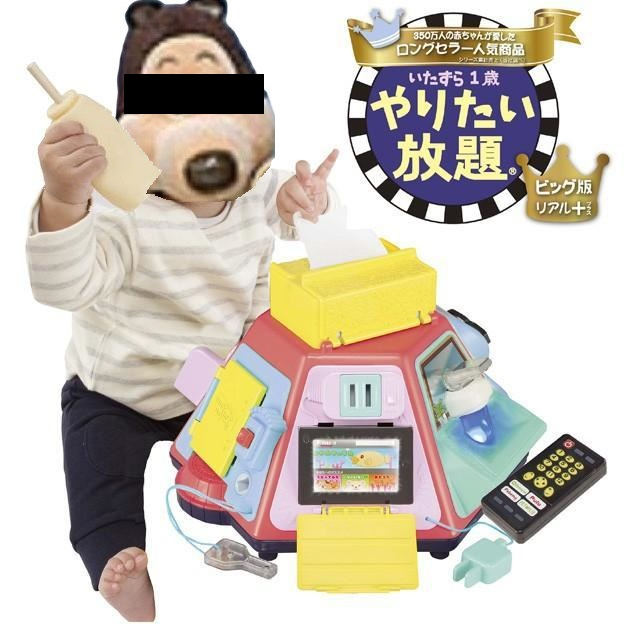
\includegraphics[width=0.25\textheight]{./FULLHOUSE/resources/1.jpg}
\end{minipage}
\begin{minipage}{\textwidth - 0.25\textheight}
  \Huge ゴロリのやりたい放題バンド\vspace{1em} \normalsize\\
    \begin{minipage}{14em}
        \Large
        tp.佐々木誇虎\\pf.沼田佳夏\\ba.野村泰成\\ds.茂木"gorori"智彦
    \end{minipage}
    \begin{minipage}{\textwidth - 15em}
        \large
        やる曲のテンポの平均がB'zの「ultrasoul」\\の倍くらいあるバンドです。\\バラードは候補にすら挙がりませんでした。
    \end{minipage}
\end{minipage}


\begin{minipage}{\textwidth - 0.25\textheight}
    \flushleft
    \Huge \vspace{1em}おげんさんといっしょ\vspace{1em}\normalsize \\
    \begin{minipage}{11em}
        \flushleft
        \Large
        pf.追川優菜\\gt.がわ\\ba.野村泰成
    \end{minipage}
    \begin{minipage}{\textwidth - 18em}
        \flushleft
        \large
        “音楽”と“だらだらお話する”のが大好きな\\
        「おげんさん一家」がみんなと一緒に\\
        「音楽で遊ぶ」バンド、それが\\
        「おげんさんといっしょ」\\
        お届けするのは「jazzyな音楽」と「急ぎめトーク」。\\
        音楽をこよなく愛するお弦3が、2Bで\\
        バンドとともに独自の視点で音楽を語ります。
    \end{minipage}
\end{minipage}
\begin{minipage}{0.25\textheight}
    \flushleft
    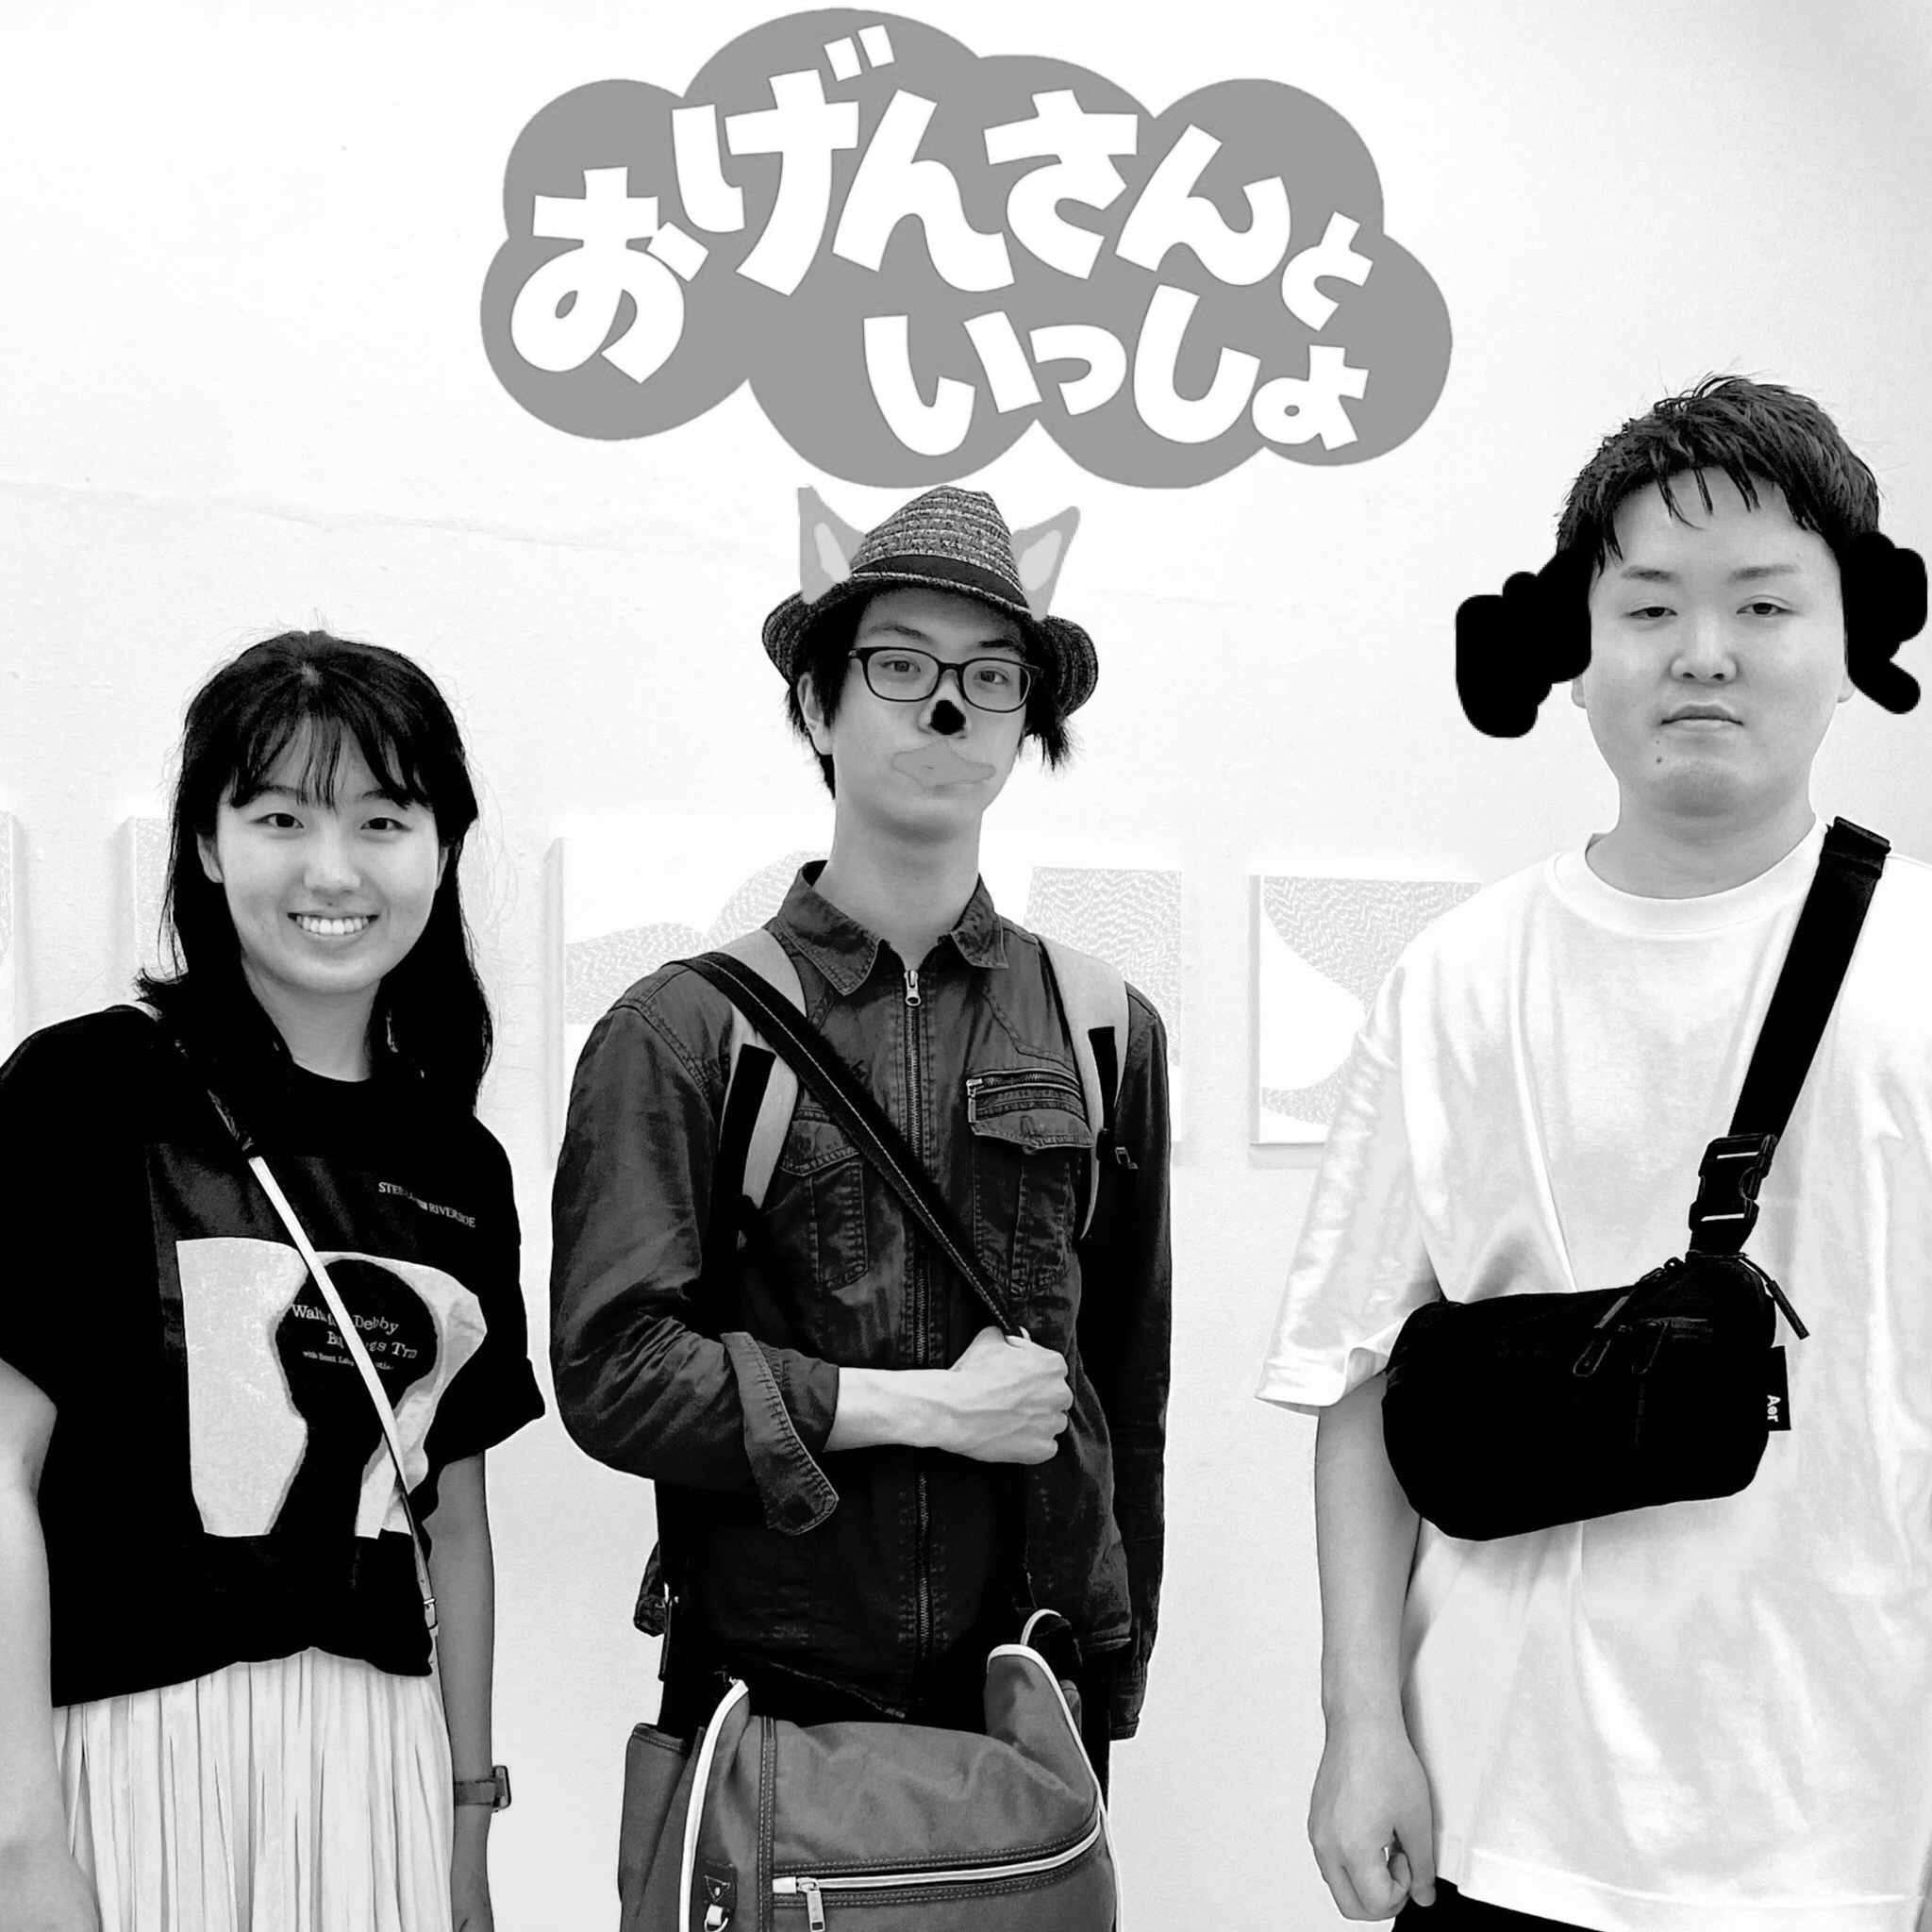
\includegraphics[width=0.25\textheight]{./FULLHOUSE/resources/5.jpeg}
\end{minipage}


\begin{minipage}{0.25\textheight}
    \flushleft
    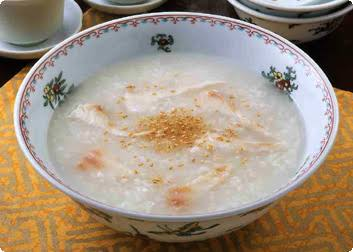
\includegraphics[width=0.25\textheight]{./FULLHOUSE/resources/6.jpeg}
\end{minipage}
\begin{minipage}{\textwidth - 0.25\textheight}
    \flushleft
    \Huge \vspace{1em}魚生粥\vspace{1em}\normalsize \\
    \begin{minipage}{11em}
        \flushleft
        \Large
        pf. 金田実樹\\tb. 大吉ひなた\\ba. 黒木崇央\\ds. 工藤ミコト
    \end{minipage}
    \begin{minipage}{\textwidth - 18em}
        \flushleft
        \large
        魚生粥(Yú shēng zhōu)は刺身を使った熱々のの中国粥。\\お粥が好きな2年生の金田と先輩達が\\熱々の演奏をお届けします。
    \end{minipage}
\end{minipage}


\begin{minipage}{\textwidth - 0.25\textheight}
    \flushleft
    \Huge \vspace{1em}ふわとろ天津班\vspace{1em}\normalsize \\
    \begin{minipage}{19em}
        \flushleft
        \Large
        Tb\&Tp.加藤玄二郎\\Cl.瀧田和佳那, Fl.中城百華\\Vo.原里伊奈, Vn.神代亜子\\Pf.長谷川和輝, Pf.片岡ゆいの\\Ba.吉田連大郎, Ba.門谷怜奈\\Dr.半澤采実, Dr.須賀敬海
    \end{minipage}
    \begin{minipage}{\textwidth - 18em}
        \flushleft
        \large
        \vspace{1em}
        おいしい天津飯の研究を頑張ってきました。なかなかの自信作です。
    \end{minipage}
\end{minipage}
\begin{minipage}{0.25\textheight}
    \flushleft
    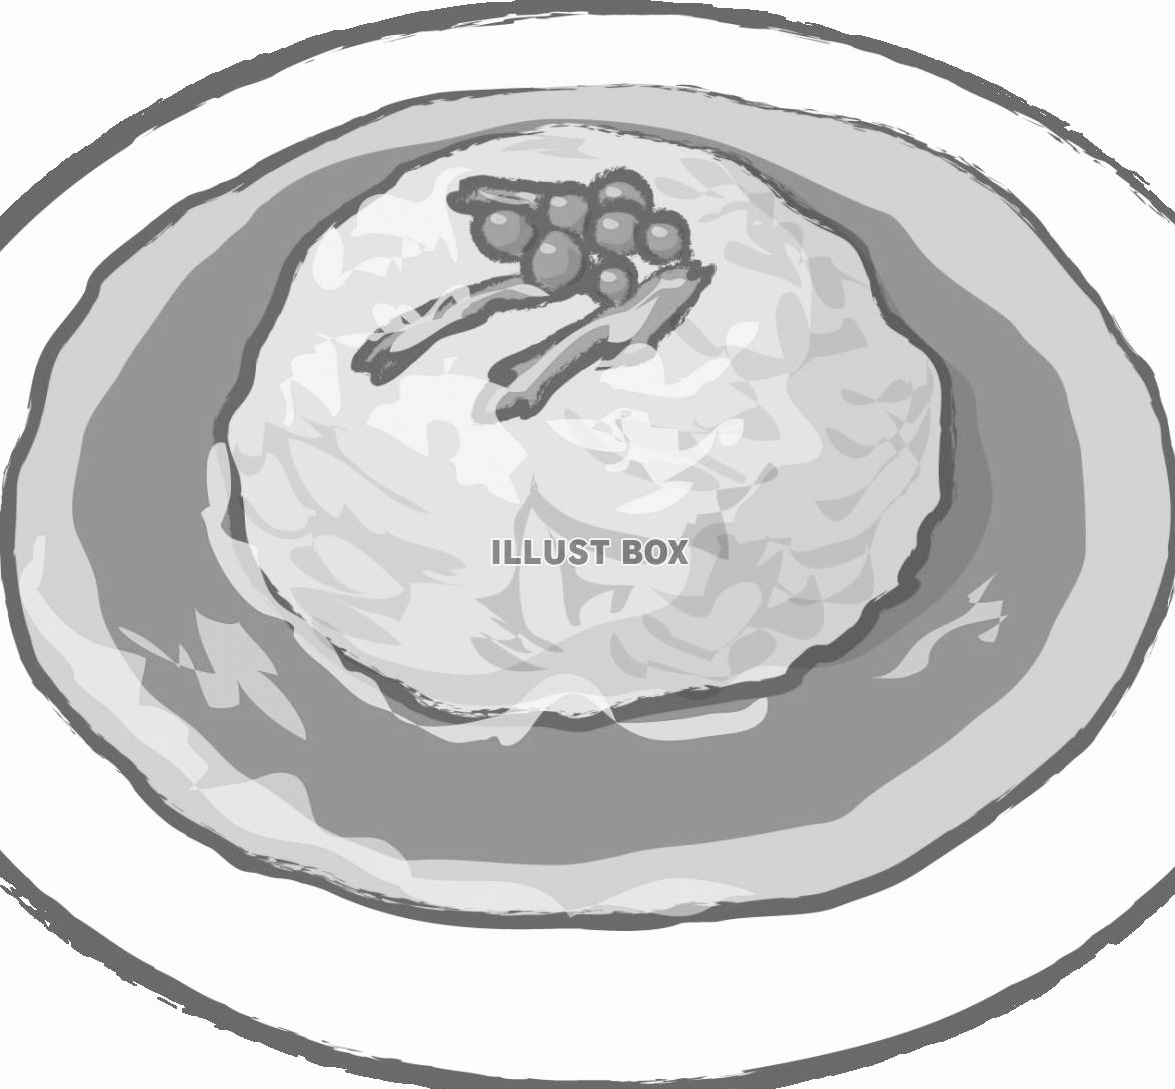
\includegraphics[width=0.25\textheight]{./FULLHOUSE/resources/8.jpeg}
\end{minipage}



\begin{minipage}{0.25\textheight}
    \flushleft
    
\includegraphics[width=0.25\textheight]{./FULLHOUSE/resources/9.jpg}
\end{minipage}
\begin{minipage}{\textwidth - 0.25\textheight}
    \flushleft
    \Huge \vspace{1em}K\&T株式会社\vspace{1em}\normalsize \\
    \begin{minipage}{15em}
        \flushleft
        \Large
        サックス.繁森有紗、北澤昴大 ピアノ.久保凜子\\ベース.亀谷旺生 ドラム.茂木智彦
    \end{minipage}
    \begin{minipage}{\textwidth - 18em}
        \flushleft
        \large

    \end{minipage}
\end{minipage}


\begin{minipage}{\textwidth - 0.25\textheight}
    \flushleft
    \Huge \vspace{1em}あんドーナツ研究会\vspace{1em}\normalsize \\
    \begin{minipage}{11em}
        \flushleft
        \Large
        vo.間瀬水也美\\as.繁森有紗\\pf.山菅昇太郎\\ba.門谷怜奈\\dr.須賀敬海
    \end{minipage}
    \begin{minipage}{\textwidth - 18em}
        \flushleft
        \large
        あなたは粒あん派?こしあん派?
    \end{minipage}
\end{minipage}
\begin{minipage}{0.25\textheight}
    \flushleft
    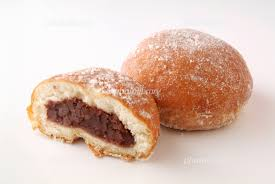
\includegraphics[width=0.25\textheight]{./FULLHOUSE/resources/10.jpeg}
\end{minipage}


\begin{minipage}{0.25\textheight}
    \flushleft
    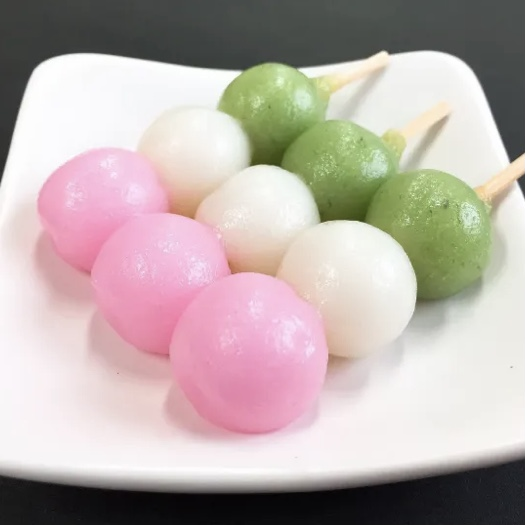
\includegraphics[width=0.25\textheight]{./FULLHOUSE/resources/11.jpeg}
\end{minipage}
\begin{minipage}{\textwidth - 0.25\textheight}
    \flushleft
    \Huge \vspace{1em}甘味一体\vspace{1em}\normalsize \\
    \begin{minipage}{11em}
        \flushleft
        \Large
        pf.内海康也\\ba.野村泰成\\dr.分銅純晴
    \end{minipage}
    \begin{minipage}{\textwidth - 18em}
        \flushleft
        \large
        ここは甘味処FULLHOUSE。\\ウェイター長もるとPA長ぶんどーがさすらいのピアニストうつみ\\と共に送るのはもちろんジャズ。\\甘ったるくもほろ苦い、あっさりしつつも\\味わい深い、そんな演奏をお届けします。\\くらえ!甘味一体!
    \end{minipage}
\end{minipage}


\begin{minipage}{\textwidth - 0.25\textheight}
    \flushleft
    \Huge \vspace{1em}無差別ティータイム\vspace{1em}\normalsize \\
    \begin{minipage}{15em}
        \flushleft
        \Large
        pf.沼田佳夏\\ba.門谷怜奈\\dr.今野陽菜
    \end{minipage}
    \begin{minipage}{\textwidth - 18em}
        \flushleft
        \large
        無差別、ゆるゆるバンドしましょ!
    \end{minipage}
\end{minipage}
\begin{minipage}{0.25\textheight}
    \flushleft
    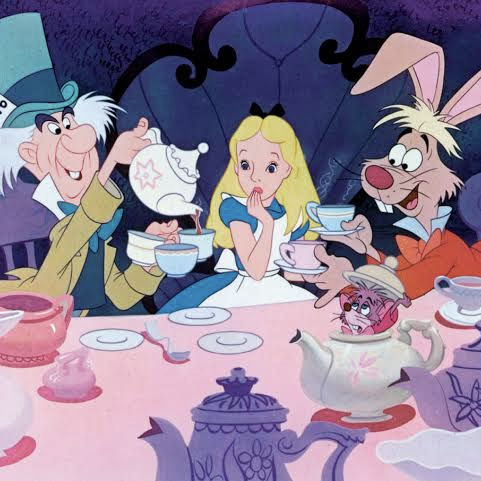
\includegraphics[width=0.25\textheight]{./FULLHOUSE/resources/13.jpeg}
\end{minipage}


\begin{minipage}{0.25\textheight}
    \flushleft
    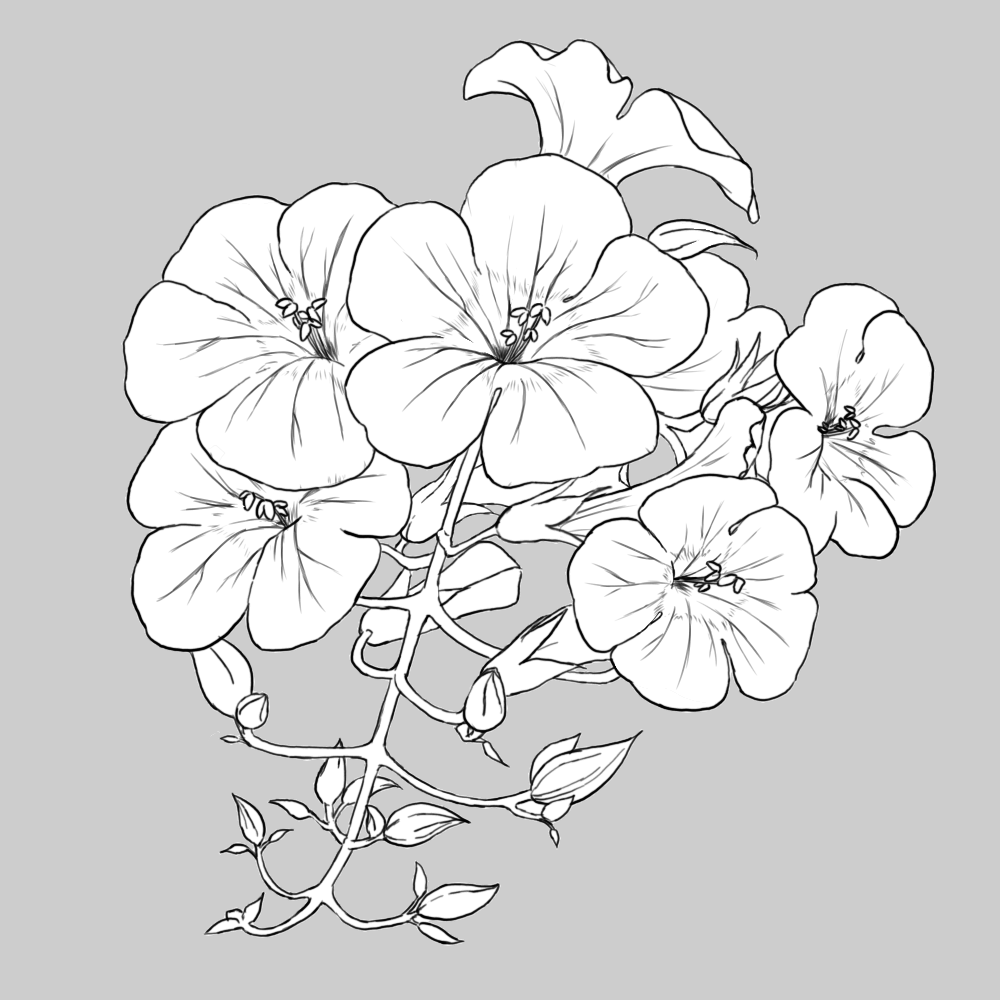
\includegraphics[width=0.25\textheight]{./FULLHOUSE/resources/14.png}
\end{minipage}
\begin{minipage}{\textwidth - 0.25\textheight}
    \flushleft
    \Huge \vspace{1em}らんまん\vspace{1em}\normalsize \\
    \begin{minipage}{15em}
        \flushleft
        \Large
        as.繁森有紗\\ pf.内海康也\\ ba.高尾真修未\\ dr.海老原梓
    \end{minipage}
    \begin{minipage}{\textwidth - 18em}
        \flushleft
        \large
    \end{minipage}
\end{minipage}


\begin{minipage}{\textwidth - 0.25\textheight}
    \flushleft
    \Huge \vspace{1em}五里霧中\vspace{1em}\normalsize \\
    \begin{minipage}{15em}
        \flushleft
        \Large
        tp.佐々木誇虎\\as.繁森有紗\\pf.山口空澄\\ba.竹内翔一朗\\ds.しばけん
    \end{minipage}
    \begin{minipage}{\textwidth - 18em}
        \flushleft
        \large
        俺たちはもう迷わない!
    \end{minipage}
\end{minipage}
\begin{minipage}{0.25\textheight}
    \flushleft
    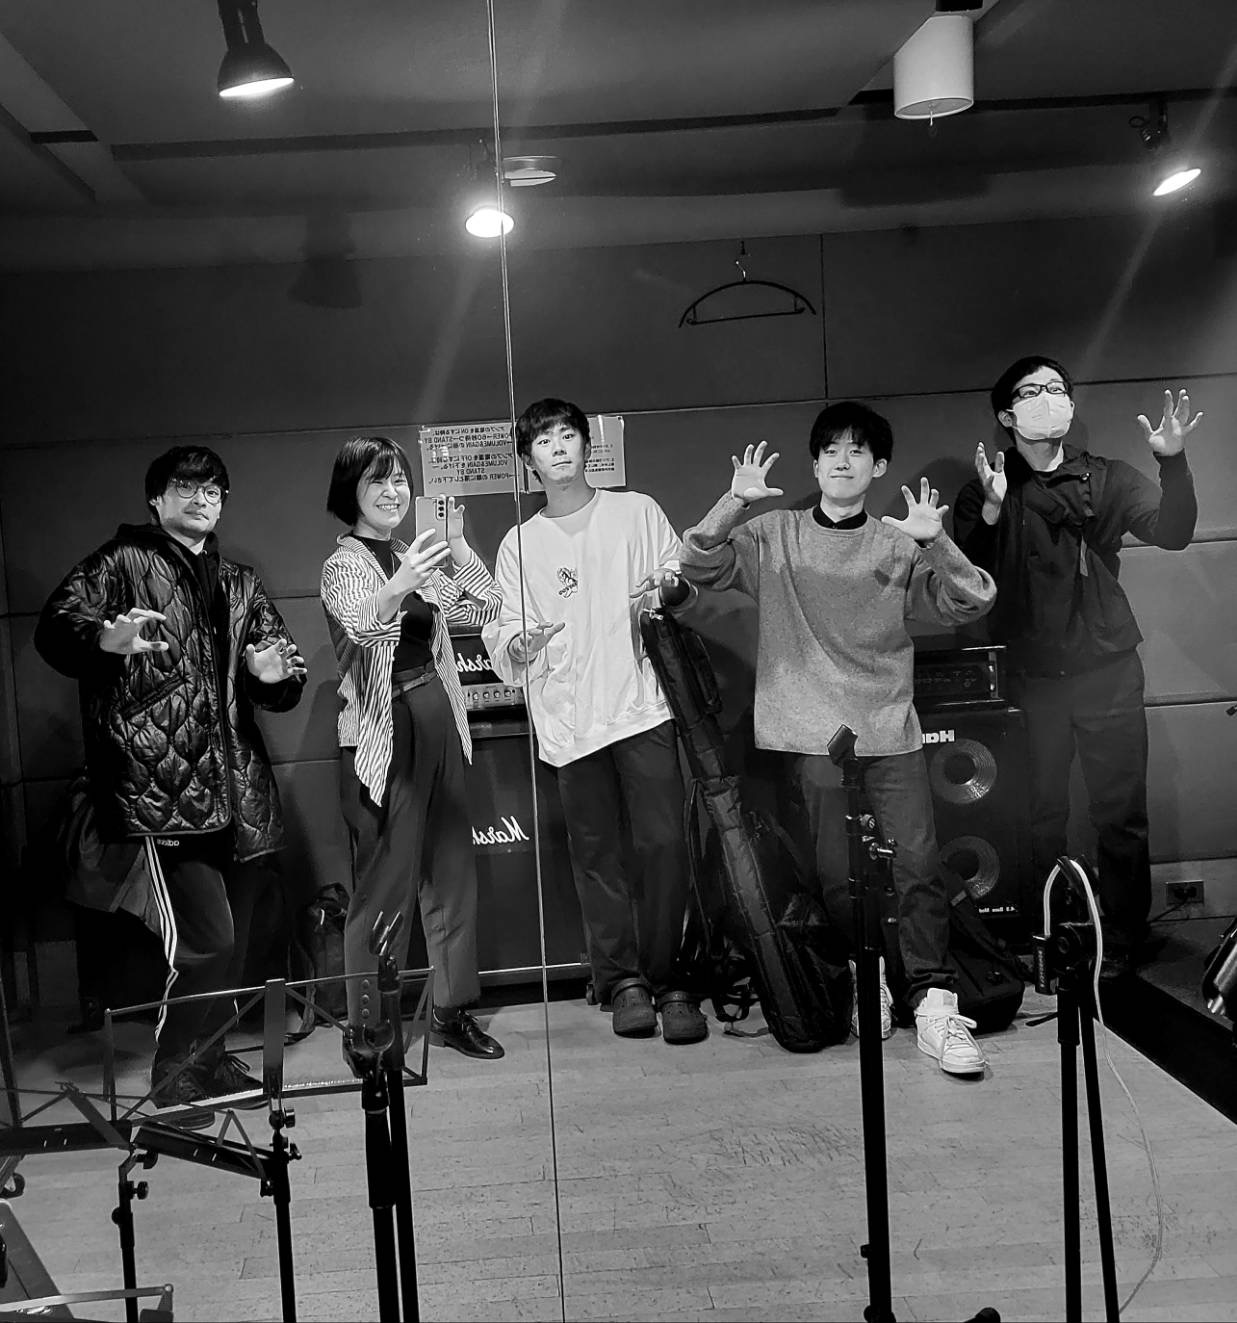
\includegraphics[width=0.25\textheight]{./FULLHOUSE/resources/15.jpeg}
\end{minipage}


\begin{minipage}{0.25\textheight}
    \flushleft
    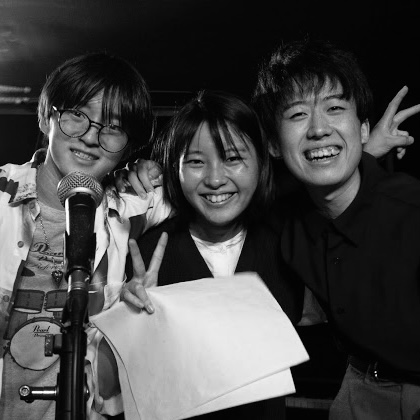
\includegraphics[width=0.25\textheight]{./FULLHOUSE/resources/16.jpeg}
\end{minipage}
\begin{minipage}{\textwidth - 0.25\textheight}
    \flushleft
    \Huge \vspace{1em}サヤインザグルーヴ\vspace{1em}\normalsize \\
    \begin{minipage}{11em}
        \flushleft
        \Large
        pf.山口空澄\\ba.渡邊千尋\\dr.分銅純晴
    \end{minipage}
    \begin{minipage}{\textwidth - 18em}
        \flushleft
        \large
        あの伝説のトリオがFULLHOUSEに帰ってくる!!
    \end{minipage}
\end{minipage}

\newpage

\begin{minipage}{\textwidth - 0.25\textheight}
    \flushleft
    \Huge 班長班\\ \huge デッドデッドデッドデッドクワガタ\vspace{1em}\normalsize \\
    \begin{minipage}{15em}
        \flushleft
        \Large
        tp/vo.畠中瑛太\\pf.岡田蒼平\\ba.渡邊千尋\\ds.工藤ミコト
    \end{minipage}
    \begin{minipage}{\textwidth - 18em}
        \flushleft
        \large
        世界を救うのは、クワガタです。
    \end{minipage}
\end{minipage}
\begin{minipage}{0.25\textheight}
    \flushleft
    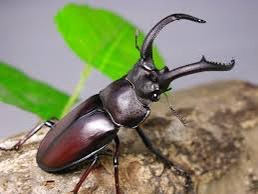
\includegraphics[width=0.25\textheight]{./FULLHOUSE/resources/20.jpg}
\end{minipage}


\begin{minipage}{\textwidth}
  \centering
  \Huge
  \vspace{3.6em}
  \begin{minipage}[t]{0.4\textwidth}
    \flushright
    店長 \\ 
    副店長 \\
    会計 \\
    調理長 \\
    副調理 \\
    PA長 \\
    副PA長 \\
    ウェイター \\
    装飾 \\
    広報 \\ 
    副広報 \\
    内装 \\ 
  \end{minipage}
  \begin{minipage}[t]{0.5\textwidth}
    \flushleft
    畠中瑛太\\
    木村惇志\\
    渡邊千尋\\
    久保凜子\\
    間瀬水也美\\
    分銅純晴\\
    亀谷旺生\\
    野村泰成\\
    今野陽菜\\
    日比野文\\
    金田実樹\\
    山口空澄\\
  \end{minipage}
\end{minipage}

\end{document}
